\section{Versuchsausfbau}
Im LHC werden zwei Protonenstrahlen auf eine Schwerpunktsenergie von $s \approx \SI{7}{TeV}$ beschleunigt und anschließend in Paketen von etwa $10^{12}$ Teilchen zur Kollision gebracht. Hierbei kommt es zu inelastischen Wechselwirkungen zwischen den Protonenstrahlen, welche in vier verschiedenen Experimenten mit unterschiedlichen Detektoren und Forschungszielen untersucht werden. Eines hiervon ist der LHCb, welcher auf die Untersuchung von $B$-Mesonen spezialisiert ist.

Das Detektorsystem des LHCb ist in Abbildung \ref{fig:Aufbau} abgebildet. Die Komponenten reihen sich in Vorwärtsrichtung hinter dem Kollisionspunkt und decken einen Polarwinkel von bis zu $\SI{300}{mrad}$ ab. Dieser Bereich ist ausreichend, da die relevanten Zerfallsprodukte in Richtung des Protonenstrahls emittiert werden.

\begin{figure}
    \centering
    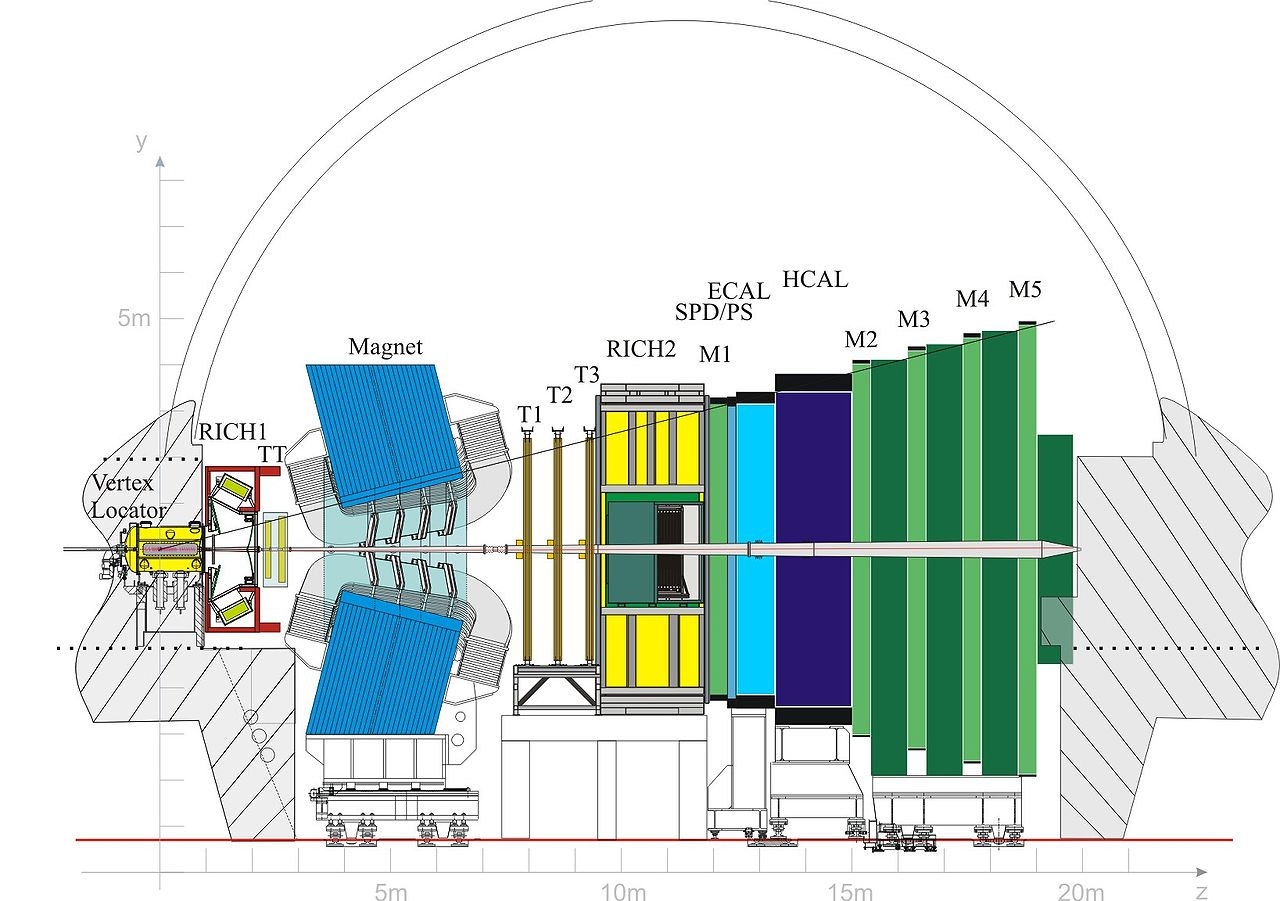
\includegraphics[width=0.7\textwidth]{plots/LHCb_Schnitt.jpg}
    \caption{Schematischer Querschnitt des LHCb Detektorsystems \cite{wiki}.}
    \label{fig:Aufbau}
\end{figure}

Um den Kollisionspunkt herum befindet sich ein Silizium-Vertex-Detektor (VELO). Die Aufteilung in viele einzelne Streifen ermöglicht die Messung der Spuren und somit die Bestimmung des Kollisionspunktes, auch Primärvertex genannt, sowie dem Zerfallsort des $B$-Mesons, dem Zerfallsvertex. Aus diesen Informationen lässt sich der Stoßparameter, der Abstand zwischen Primär- und Zerfallsvertex, bestimmen.

Anschließend ist ein Ring-Imaging-Cherenkov-Detektor (RICH) zur Geschwindigkeitsbestimmung positioniert, welcher zur Teilchenidentifikation genutzt wird. Teilchen, welche sich mit einer Geschwindigkeit durch den Detektor bewegen, welche höher als die Lichtgeschwindigkeit des durchquerten Mediums ist, emittieren Cherenkovstrahlung, welche von umliegenden Photodioden registriert wird. Als Medium werden ultraleichte Festkörper oder Gas verwendet. Über den Abstrahlwinkel der Strahlung lässt sich die Geschwindigkeit des Teilchens berechnen.

Es folgt ein weiterer Siliziumstreifendetektor (TT) mit einer größeren Fläche als der VELO. Dieser dient zum einen zur Spurrekonstruktion von niederenergetischen Teilchen, welche durch das anschließende Magnetfeld zu stark abgelenkt werden, um weiter detektiert zu werden. Im Anschluss befindet sich ein Dipolmagnet, dessen Magnetfeld die geladenen Teilchen auf eine gekrümmte Bahn ablenkt. Aus der Kombination der Spuren des TT und der darauffolgenden Spurdetektoren (T1, T2, T3) kann die Krümmung der Spur bestimmt werden.
Aus dem Krümmungsradius kann anschließend der Impuls berechnet werden. Als Spurrekonstruktionsstationen $T_\mathrm{i}$ werden weitere Siliziumstreifenmodule, sowie Proportionalzählrohre verwendet.

Daraufhin folgt ein weiterer RICH-Detektor und ein Kalorimetersystem. Letzteres ist aus einem Scintillating Pad (SPD), einem Preshower-Detektor (PS), einem elektromagnetsichen (ECAL) und einem hadronischen Kalorimeter (HCAL) zusammengesetzt. Die Kalorimeter bestehen aus abwechselnden Schichten von Absorbern und Szintillatoren, sodass die Teilchen in den entsprechenden Kalorimetern schauern und vollständig absorbiert werden. Die Anzahl der Schauerteilchen ist hierbei proportional zur Energie des Teilchens.

Da Myonen zu den minimal ionisierenden Teilchen gehören, werden diese jedoch nicht im Kalorimetersystem absorbiert. Aus diesem Grund befindet sich zuletzt ein System aus Myonenkammern (M1 bis M5), welche aus abwechselnden Schichten von Eisenabsorbern und Vieldrahtkammern bestehen. Sie dienen zur Identifikation der Myonen, da nur diese den gesamten Detektor durchqueren und ein Signal in den Myonenkammern erzeugen. \cite{lhcb}, \cite{lhcbpaper}, \cite{lhcbmachine}

\section{Datenaufnahme}
Die im Versuch verwendeten Daten stammen aus Proton-Proton-Kollisionen aus dem Jahr 2011 mit einer Schwerpunktsenergie von $\sqrt{s}=7\;\si{TeV}$. Unterschieden wird zwischen zwei Datensätzen mit unterschiedlicher Magnetfeldpolarisation, um den Effekt uneinheitlicher Detektionseffizienzen von Teilchen umgekehrter Ladung zu vermeiden. Teilchen mit entgegengesetzten Ladungen werden durch das Magnetfeld in verschiedene Detektorbereiche abgelenkt, welche voneinander leicht abweichende Wechselwirkungsquerschnitte haben und so die Asymmetriemessungen verfälschen können.

Aus dem Detektorsystem wird eine große Anzahl an Informationen gewonnen, welche aufgrund der hohen Datengröße schwierig zu verarbeiten ist. Außerdem sind nicht alle Informationen relevant für die physikalischen Untersuchungen. Aus diesem Grund werden die Daten mit Hilfe eines Systemes zur Datenselektion, auch Trigger genannt, bearbeitet.
Mittels der Informationen aus den Teilchenidentifikationssystem wird das Ereignis vollständig rekonstruiert und die beteiligten Teilchen identifiziert. So können uninteressante Zerfallskanäle und Hintergrundsereignisse aussortiert werden. Des Weiteren werden die Messdaten auf für die Untersuchung relevante Observablen reduziert. 

In der Arbeitsgruppe der Technischen Universität Dortmund wird durch weitere Selektionen der Untergrund der Daten erneut reduziert. Hierbei sollen die Daten auf den $B^{\pm}\rightarrow h^{+}h^{+}h^{-} $ Zerfall zugeschnitten werden. Als Selektionsvariable wird zum einen der Impuls der Endzustandsprodukte verwendet, welcher einen Betrag im GeV-Bereich haben soll. Des Weiteren wird aus den Zerfallsprodukten die Masse des Primärteilchens bestimmt und auf einen Bereich um die Masse des $B$-Mesons herum zugeschnitten. Außerdem wird der Stoßparameter, der Abstand zwischen Primär- und Zerfallsvertex, aufgrund der kurzen Lebensdauer des $B$-Mesons auf kleine Werte festgelegt.

Zum Vergleich werden des Weiteren Simulationen angefertigt, welche sowohl das physikalische Verhalten als auch die Detektorantworten darstellen können. Für diesen Versuch stehen allerdings lediglich die Erstgenannten zur Verfügung. \cite{anleitung}
